pr%************************************************
\chapter{Middleware}\label{ch:middleware}
%************************************************
\section{Introduction}\label{sec:mwintro}
Once an application or sub-domain has been modelled it is necessary for software to interact with the triple-store to make use of that data. This currently requires specialist knowledge, not common in the software engineering community and which presents another barrier to adoption of ontology in the rail domain. In particular interacting with a triple-store requires knowledge of the following specific technologies as a minimum:
\begin{itemize}
    \item SPARQL
    \item XML data types 
    \item The triple store interface: typically either a library or a network protocol
\end{itemize}

Additionally in order as for the knowledge of the specific technologies to be of value a certain amount knowledge of higher level ontology principles is required. At the very least a familiarity with triples and, in an environment where reasoning is used, inference is also required. It is reasonable to expect that a software engineer will have some knowledge of XML data types and learning the correct way to interface with the triple store would also be accomplished within the time frame available to most large projects, learning SPARQL or higher level concepts will take significantly longer.

Whilst it is possible in the long term that this skills gap will be filled by education in the short and medium term the adoption of ontology linked data in the rail domain would be considerably accelerated by allowing software engineers without ontology specific knowledge to interact with data stored in an ontology. The RaCoOn middleware bridges that gap.

The RaCoOn middleware, as the name implies, exists as an intermediary between the triple store holding the ontologies and applications needing to access it. Beyond making connection possible the middleware also handles connections to REDIS, for high frequency data, and adds a security layer. Consuming applications are presented with Windows Communication Foundation, here on refereed to as WCF, web services implementing, where possible, RESTFul design principles. This middleware makes several contributions to ontology development for the railways: Firstly it acts as a \say{cut-out} between the triple store and the consumer. Different project consumers will need to access triple stores in different ways and as the market evolves it is possible, even likely that different triple stores will be used. The middleware insures that as the components on either side change the larger system is unaffected. The same interface will be presented to the consumer regardless of the triple store. Another key benefit is the ability to integrate different data stores, beyond the triple stores such as STARDOG. Currently REDIS is available for high frequency data, however as and when other data-stores are identified as bringing value to a project they can be integrated without changing the existing set-up. Since some data stores don't have their own security, an additional benefit of the middleware is a single sign on and token system can be handled by the middleware. Another key benefit of the middleware is that common functions can be included in the middleware, avoiding the need to create them repeatedly in client applications. Additionally it is possible to connect to the middleware using clients written in most common languages and from most environments, allowing developers to use the best tool for the current project. The overall architecture is summarised in \autoref{fig:MiddlewareHighLevel}.

As discussed in \autoref{ch:litreview} a major challenge when moving from the current ecosystem of mixed incompatible data stores to one that embraces linked data and ontology, is that of data volumes. Whilst the market has moved forward significantly and there now exist many triple stores capable of scaling to deal with high volume data, when run in an appropriate environment, triples are fundamentally not the most memory efficient way of storing data. When using RaCoOn high frequency data can be stored separately in more appropriate stores, such as REDIS\footnote{REDIS is an open source project, more details are available from: \url{https://redis.io/}}, as discussed by \citet{Tutcher2015} in chapter six. When dealing with very high volume and velocity data representing it as triples is sometimes impractical, even with cloud-scale computing available. At these times it is necessary to add the data to an external store and put a summary of that data in the triple store along with a link which can be used to retrieve it. For example where a complex wave form is recorded, it's amplitude, duration and the time and which the sample was taken could be stored as triples, alongside a key to retrieve it from a key-value type store such as REDIS. Is highly optimised for fast retrieval of large amounts of data using a very simple key, deliberately leaving security to entirely the user, as such if you can connect to the server and know the key of the item it will return it.

 \begin{figure}[!h]
\myfloatalign
{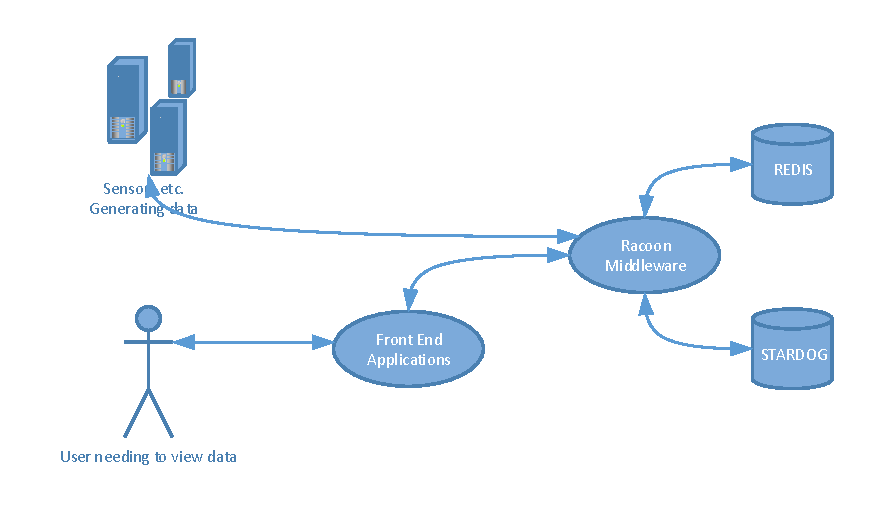
\includegraphics[width=\linewidth]{gfx/Middleware}} 
\caption{The role of the Middleware}
\label{fig:MiddlewareHighLevel}
\end{figure}

\section{Functionality}

In order as to fulfil the role described in \autoref{sec:mwintro} the following functionality must be implemented. 

\subsection {Intermediary}
The middleware must act as an intermediary between consuming applications, source applications and data stores. One of the challenges faced during the transition to linked data is that of the triple stores available changing with time, alongside the interfaces they present as new technologies are developed and standards are created. Client applications will be created on an as needed basis when a project requires them over a number of years, no \say{big bang} style creation event is foreseen in which the entire industry is migrated over to linked data over night. As such different triple stores and different interfaces to the same triple store will need to be used. 

Suppliers are starting to respond to the industries' need for easier to use interfaces to triple stores and SQARQL has existed as a constantly evolving standard query language for some time, however this does not alleviate vendor lock in when choosing a triple store. 

\subsection{Datastore aggregation}
New data stores being developed rapidly as the technology matures, all with different strengths and weaknesses. NoSQL data stores in particular are gaining market traction and \citet{Moniruzzaman2013} reviews them. As the market evolves it is possible, even probable, that new projects will require access to different types of data store, in keeping with the project's needs. In the first instance REDIS has been selected as a second data store to make available, since this has been used in previous projects with RaCoOn for high frequency data. In particular in the FuTRO project, reported in \cite{Tutcher2013}, REDIS was used to hold very high frequency sensor data. Many railway condition monitoring applications, such as alternating current field measurement (Heron: ACFM) sensors or laser distance sensors, as used in condition monitoring of railway assets can generate very high volumes of data for example \citet{Rowshandel2013}, which used the sensors discussed mounted on a robotic arm, to find cracks in rails. 

\subsection{Stored Procedures}
The middleware provides \say{Stored Procedure} functionality similar to that commonly found in relation databases, which have several benefits, applicable to both relational data stores and this system:

\begin{itemize}
    \item Familiarity for developers used to a relational database environment. 
    \item Improved reuse. Once a stored procure has been written it can be used by many systems, or the same system in many places with out rewriting it;
    \item Less data needs be sent to the middleware since the name of the stored procedure is much shorter than the SPARQL required to describe the query; 
    \item Isolation between the software and the query. As such if the representation of the data changes only the query need change, not the system using it. In the case of ontologies, as opposed to relational databases, this should only be relevant if major re-factoring is done for example if a different domain had to be used for all URI's in the system.
\end{itemize}

By providing a familiar mechanism to developers coming from a relational database background, common to many developers both within in the railway domain and in the broader software engineer community it is possible to reduce the learning curve for a new technology. Other benefits from the relational database domain are less applicable to the linked data domain, in particular the stored procedures can't be stored pre-compiled for faster execution since the middleware is not responsible for the compilation of the query.

 Stored procedures created in the middleware can seamlessly use any datastore, there is no difference to the user and no changes to the implementation need be made when a different store is used, though it is probable the stored procured will need to be updated to match the new store. Code which has been developed to use one data store via the middleware can of course continue to do so when another is added. 

\subsection{Security}
The middleware provides security for those data stores that do not include security themselves and implements a token system to avoid the need for storing passwords on client machines.

\subsection{functionality moved to the middleware}\label{midfunc}
Functionally that will be used repeatedly across multiple projects has been moved to the middleware that easing the development burden in future projects. Aside from the expected functionality to handle security and to query the data stores the middleware connects to, both using store procedures and queries the following functionality has been added:
\begin{itemize}
    \item Free text search of individuals within a class, using the label text;
    \item Get all individuals of a given type;
    \item Add new items;
    \item Load Layout definition files - a file format describing rail infrastructure.
\end{itemize}

\subsection{Interoperability}
Another challenge to the take up of ontology and linked data in the rail domain is that of the number of unique interfaces presented by each different datastore, the Middleware conversely presents clients with web-services, which will not need to be re-learnt when new data stores are added. Whilst these are implemented in WCF, which is traditionally consumed by clients written in .Net however the services are described using a standard XML Web Service Definition Language (WSDL) document, which most commonly used languages have tools and libraries for making use of. 

\section{Design}
As with the schedule parsing tool set out in \autoref{ch:cifparser} this system was designed in an object orientated manor and made heavy use of inheritance. SOLID\footnote{A good explanation of SOLID design principles, illustrated with motivational posters, may be found at \url{https://blogs.msdn.microsoft.com/cdndevs/2009/07/15/the-solid-principles-explained-with-motivational-posters/}} software design principles, as first set out by \citet{Martin2003}, were employed. 
\subsection{High Level}
The middleware solution contains the following projects:

\begin{description}
    \item[RacoonMiddleware] Holds the Webservices and calls the other projects as needed;
    \item[MiddlewareBussinessObjects] Holds representations of objects referred to by the ontology as C\# objects;     
    \item[REDISConnector] Acts as the intermediary between the middleware and REDIS.
    \item[StoredProcCreator]
    This module compiles to provide a simple win32 interface for creating and editing stored procedures. 
    \item[StardogConnection]  Acts as the intermediary between the middleware and Stardog.    
    \item[UploadLDLTool]
    This module compiles to a very simple Wind32 tool for testing the processing of LDL files, required for a specific project which is set out in  \autoref{ch:COMPASS}. It is not intended for production use, rather it was a debuging tool before the functionality had been added to another system.
    \item[UserManager]
    This tool manages the users that have access to the middleware. It is a small, simple tool for use by system administrators.
\end{description}

\subsection{Details}
\subsubsection{RacoonMiddleware}
This project contains the webservice definitions and the functionality directly related to them and thus is the part of the project with which external developers will interact directly. In particular it contains definitions of all the responses that can be given by the webservices and all the parameters accepted.

This project in particular makes heavy use of object orientated design and inheritance. All of the responses returned by the webservice extend a simple base class entitled \say{\texttt{SimpleRacoonResponse}}, which provides the basic details every response from the webservice will include, namely:
\begin{description}
    \item[AuthorisationOK] A Boolean value indicating if the token provided was accepted. If this is false then the token is not valid. The most probable cause for this is the token timing out, since they are only valid for a given length of time, currently configured as one hour.
    \item[Error] An exception, if this is not null an error of some kind has occurred. The message should be disable to a user and the type of the exception should be informative.
    \item[Status] If this is true the operation completed successfully and the results can be replied upon. If it is false then the results should be discarded. 
\end{description}

This inheritance is set out in \autoref{fig:MiddlewareResponses}, which also gives details of the possible response types. The response classes in turn all either implement one of the interfaces set out in \autoref{fig:ResponseInterfaces} or a extend a class that does. This was in keeping with good object orientated design practice, since every response will need to return certain functionality and it allows the system both handling and generating those responses to be written once, not rewritten for every webservice. This design principle extends well beyond web services for accessing ontologies, it can be beneficial for any system offering numerous similar webservices. Inheritance was also used by the classes implementing the webservices, in keeping with the principles of reusing code rather than copying it, as shown in \autoref{fig:services}.

 \begin{figure}
\myfloatalign
{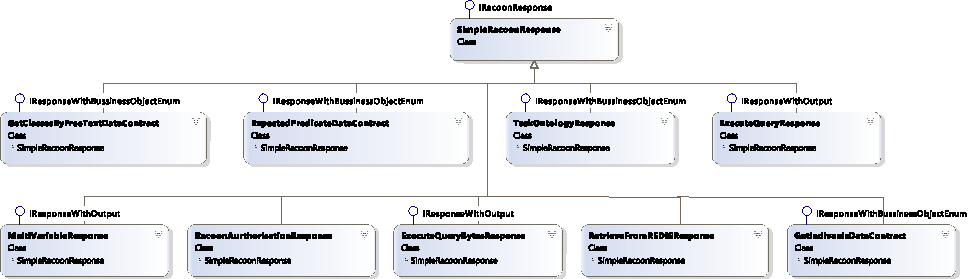
\includegraphics[width=\linewidth]{gfx/MiddlewareServicesClassesResponseOnly}} 
\caption{The response types returned by the RaCoOn Middleware}
\label{fig:MiddlewareResponses}
\end{figure}

 \begin{figure}
\myfloatalign
{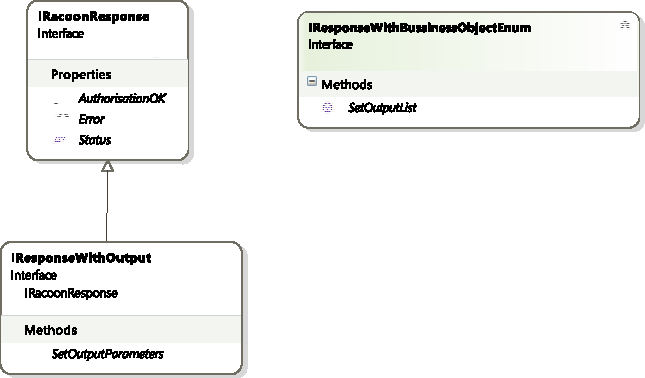
\includegraphics[width=\linewidth]{gfx/Res}} 
\caption{The interfaces implemented by webservice responses}
\label{fig:ResponseInterfaces}
\end{figure}

 \begin{figure}
\myfloatalign
{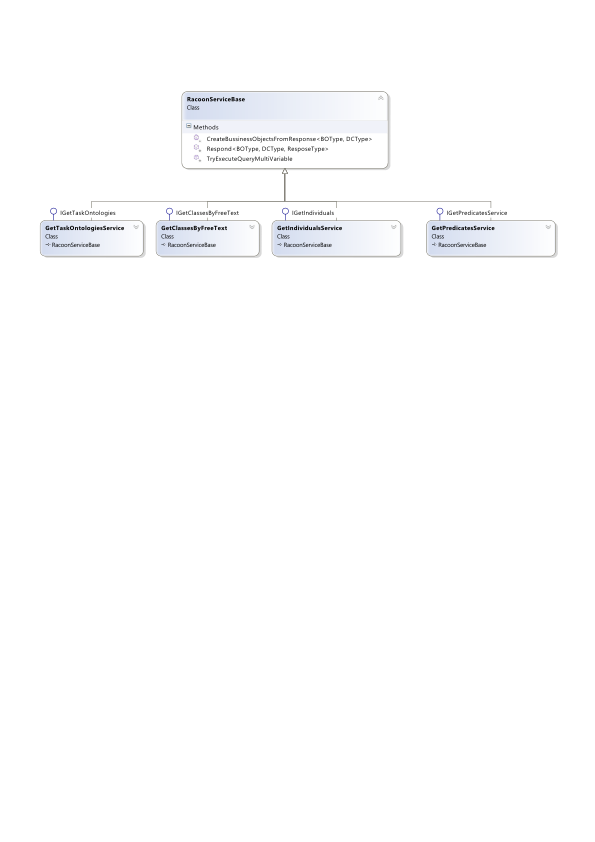
\includegraphics[width=\linewidth]{gfx/RacoonServices}} 
\caption{Selected webservices}
\label{fig:services}
\end{figure}

This module is also responsible for acting as a \say{cut out} between multiple different data stores. Whilst only REDIS and stardog functionality are currently implemented the framework is flexible and would allow for the addition of extra datastores with no impact on the existing stores or the framework. All that is necessary is the addition of a Dynamic Link Library, here on referred to as a DLL and stored procedures using that datastore can be executed. The DLL must export a class which implements the interface set out in \autoref{lst:query}. Stored procedures have a field setting out the fully qualified name of the stored procedure's type, as seen in \autoref{lst:StoredProcedure} so if the DLL is in memory all that needs be done to access a new datastore is create a stored procure with that type specified and it will be used, with no code changes to this module. This has several benefits; firstly isolation between the datastore specific code, which is prone to change in order as to match changing data store interfaces, secondly it reduces the amount of testing that need be done when new data stores are added and lastly it allows for adding new datastores without needing a full understanding of the RacoonMiddleware.

\begin{lstlisting}[language={[Sharp]C},frame=tb,caption={The IQuery interface, which must be implemented by all executable queries},label=lst:query]
/// <summary>
/// An abstract query, targeting any data store. Includes methods for setting any variables included in the query
/// </summary>
public interface IQuerry
{
    void SetTarget(string server,string datastore);
    void SetQuerry(string queryText);
    IEnumerable<MiddlewareParameter> Execute(IEnumerable<MiddlewareParameter> parameters, Session session, ParameterTypeEnum returnTypeWanted);      
}
\end{lstlisting}

As can be seen from \autoref{lst:query} queries and stored procedures can take any number of parameters, which can be one of several types:

\begin{description}
    \item[String] String data and all other data types not specifically handled;
    \item[Uri]  Unique Resource Identifiers, as used in linked data;
    \item[Byte] For transferring binary data.
\end{description}

This list can be expanded if needed. These restrictions only apply to stored procedures and to functions directly passing queries. Task specific Webservices can take or return any type including a business object related to the operation they perform, or a simple in built types.

Stored procedures are also handled by this module, \autoref{lst:StoredProcedure} shows it's implementation.

\begin{lstlisting}[language={[Sharp]C},frame=tb,caption={The StoredProcedure class. Constructors, private fields and utility methods have been omitted for brevity.},label=lst:StoredProcedure]
 public class StoredProcedure
    {              
        private void createQuery()
        {
            lock (theQueryLock)
            {                
                //Cause the exception to be thrown here if the type doesn't exist, for clarity sake.
                Type queryType = Type.GetType(TypeOfQuerry, true);
                TheQuerry = Activator.CreateInstance(queryType) as IQuerry;
                if (TheQuerry == null)
                    throw new InvalidOperationException("The Query is not of a valid type");
                TheQuerry.SetTarget(Server, DataStore);
                TheQuerry.SetQuerry(StoredProcText);
            }
        }

        /// <summary>
        /// A hash of the storedproc name, used as a key to retrieve it
        /// </summary>
        public int KeyHash;

        /// <summary>
        /// The executable version of the query
        /// </summary>
        [XmlIgnore]
        public IQuerry TheQuerry
        {
            get
            {
                if (theQuery == null) createQuery();
                return theQuery;
            }
            private set
            {
                theQuery = value;
            }
        }

        /// <summary>
        /// The server at which the stored proc is targeted. Where this is null or empty the value from the Session is used
        /// </summary>
        public string Server;
        /// <summary>
        /// The Datastore at which the stored proc is targeted. Where this is null or empty the value from the Session is used
        /// </summary>
        public string DataStore;
        /// <summary>
        /// The name of stored proc
        /// </summary>
        public string Name;
        /// <summary>
        /// This is the name of the type of query to instantiate 
        /// </summary>
        public string TypeOfQuerry;
        /// <summary>
        /// The text of the command e.g. SELECT * WHERE {?s ?p ?o}
        /// </summary>
        public string StoredProcText;
    }
\end{lstlisting}

An XML file, holding numerous instances of the class shown in \autoref{lst:StoredProcedure} provides the database of stored procedures. For efficiency this is read into a dictionary in memory on start-up then stored procures are retrieved, using a hash of the stored procedure's name as it's key in the dictionary. This allows for very fast access to stored procedures, which is necessary when dealing with high velocity data, such as that from sensors.



\subsection{MiddlewareBussinessObjects}

This project is compiled as a DLL, to allow for it's reuse in other projects and to keep coupling between the business objects and the implementation of the webservices loose. Modelling concepts stored in an ontology as objects in a programming language makes manipulating them more intuitive, both for external users and for developers working on the middleware. There exist frameworks to automatically generate objects from classes held in various triple stores\footnote{the open source project JENA has this capability}, however, at the time this was project was developed none were available for C\# as such this development was done manually.

 Moving from the ``Open World'' of RDF and ontologies to Object Orientated languages does require the developer (or the designer of the tool, where this is automated) to make some decisions as to how classes and properties are modelled as objects and properties. In the case of \say{Object Properties}, that is properties that \say{connect pairs of individuals} as specified in \citet{McGuinness04}, representation as an object is possible, so long as both the individuals to be linked are of types modelled in the system. Unless there are cardinality restrictions, such as marking a property as functional, then a list or similar collection class, is appropriate to link objects, unless the developers domain knowledge rules out this possibility. For example when linking objects of type train and driver, via an object property of type ``currentDriver'' it would be unnecessary to use a list, even if the property has not had any cardinality restrictions placed upon it to reduce the amount of reasoning required. This is illustrated in \autoref{lst:bgtob} which shows the relationship between Balises and Balise Groups. Cardinality restrictions require checking when an object is inserted and thus represent a (small) performance cost. Further more in the most restrictive of decision logics they are not available. If a property is marked as functional, that is it uses the type \texttt{owl:FunctionalProperty}, then an individual can have at most one value for that property and thus there is no need to use a list to link them.

\begin{lstlisting}[language={[Sharp]C},frame=tb,caption={Linking of Balises to BaliseGroups},label=lst:bgtob]
   public List<LDLBalise> Balises;
\end{lstlisting}

 Another way in which business objects were employed in the the middleware was modelling source data sets for insertion into the ontology. As discussed in \autoref{ch:cifparser} the rail industry has many data sources in a variety of formats and in order as to insert them into the ontology it is necessary first to represent the data they hold as simple objects, then to iterate over a collection of these objects inserting them into the data store.

In the case of \texttt{Dataatype properties}, also known as value properties, all that need be done generally is adding a public field of the appropriate type to the object. The datatypes are restricted to inbuilt XML data types, which closely align with the available datatypes in most programming languages. 

\subsection{Stardog Connector}

The stardog connector module is an example of a how a data source can be interfaced with the middleware. In particular this module shows how a triple store can interact with the middleware and then client applications. This module exports a Query, compliant with the \texttt{IQuery} interface defined in \autoref{lst:query} allowing the RacoonMiddleware to query this data store. The dependencies directly pertaining to stardog are imported in this module. Should they require updating (as they periodically do) then only this module requires recompilation.

\subsection{REDIS Connector}

This performs the same role as the Stardog Connector, further demonstrating that middleware can aggregate multiple datastores.


\subsection{Other Modules: StoredProcCreator,UploadLDLTool, and UserManager}
The other modules differ from those above in that they compile into executable programs in there own right. These tools provide examples of the supporting tool chain that is required to accompany any means of connecting users to datastores. A single unified log on is desirable, thus user management is required, especially when some data stores have no security. Whilst it is possible to create stored procedures by hand, requiring it would simply be another barrier to use as such it is desirable to create a simple user interface to enable this. 

Note that each of these programs imports other units from across the project.
\section{Results}
*****Including verifiation